\pagebreak
\section{Geometría}
\def\svgwidth{\columnwidth}
\subsection{Circunferencia y Círculo}
Dado un punto $O$, y una distancia $r$, la circunferencia está definida por el conjunto (infinito) de todos los puntos en el plano que están a una distancia $r$ de $O$. Un círculo corresponde a la circunferencia junto con la región inscrita dentro de ella.\\

\subsubsection{Ángulos de una Circunferencia}
\textit{Ángulo de Centro:} Vértice en el centro, sus lados son dos radios.\\
\textit{Ángulo Interior:} Vértice dentro de la circunferencia (no en ella!), sus lados son dos cuerdas.\\
\textit{Ángulo Exterior:} Vértice fuera de la circunferencia, sus lados son dos secantes, una secante y una tangente, o dos tangentes.\\
\textit{Angulo Inscrito:} Vértice en la circunferencia, los lados son dos secantes o cuerdas.\\
\textit{Ángulo semiinscrito:} Vértice en la circunferencia, un lado secante y otro tangente.\\

\subsubsection{Teoremas de Ángulos}
Unidades: $360^{\circ} = \SI{2\pi}{\radian}$\\

Con $\angle ACB$ inscrito y $\angle AOB$ de centro,
$\measuredangle ACB = \frac{\measuredangle AOB}{2}$.\\

Análogamente, con $\angle ABC$ semiinscrito (tangente), y $\angle BOC$ de centro, $\measuredangle ABC = \frac{\measuredangle BOC}{2}$.\\

La medida de un \textbf{ángulo interior} es igual a la semisuma de las medidas angulares (de centro) de los arcos formados por dicho ángulo:
\begin{equation*}
    \measuredangle APB = \frac{m(\stackrel\frown{AB}) + m(\stackrel\frown{CD})}{2}
\end{equation*}
Con $\angle APB$ interior, y $\stackrel\frown{AB}$ y $\stackrel\frown{CD}$ arcos formados por el.\\

De la misma forma, la medida de un \textbf{ángulo exterior} es igual a la semidiferencia de los ángulos de centro formados por el ángulo. (mayor primero)
\begin{equation*}
    \measuredangle APB = \frac{m(\stackrel\frown{AB}) - m(\stackrel\frown{CD})}{2}
\end{equation*}

\subsubsection{Teoremas de Trazos}
\textbf{Teorema de las Cuerdas}\\

\begin{center}
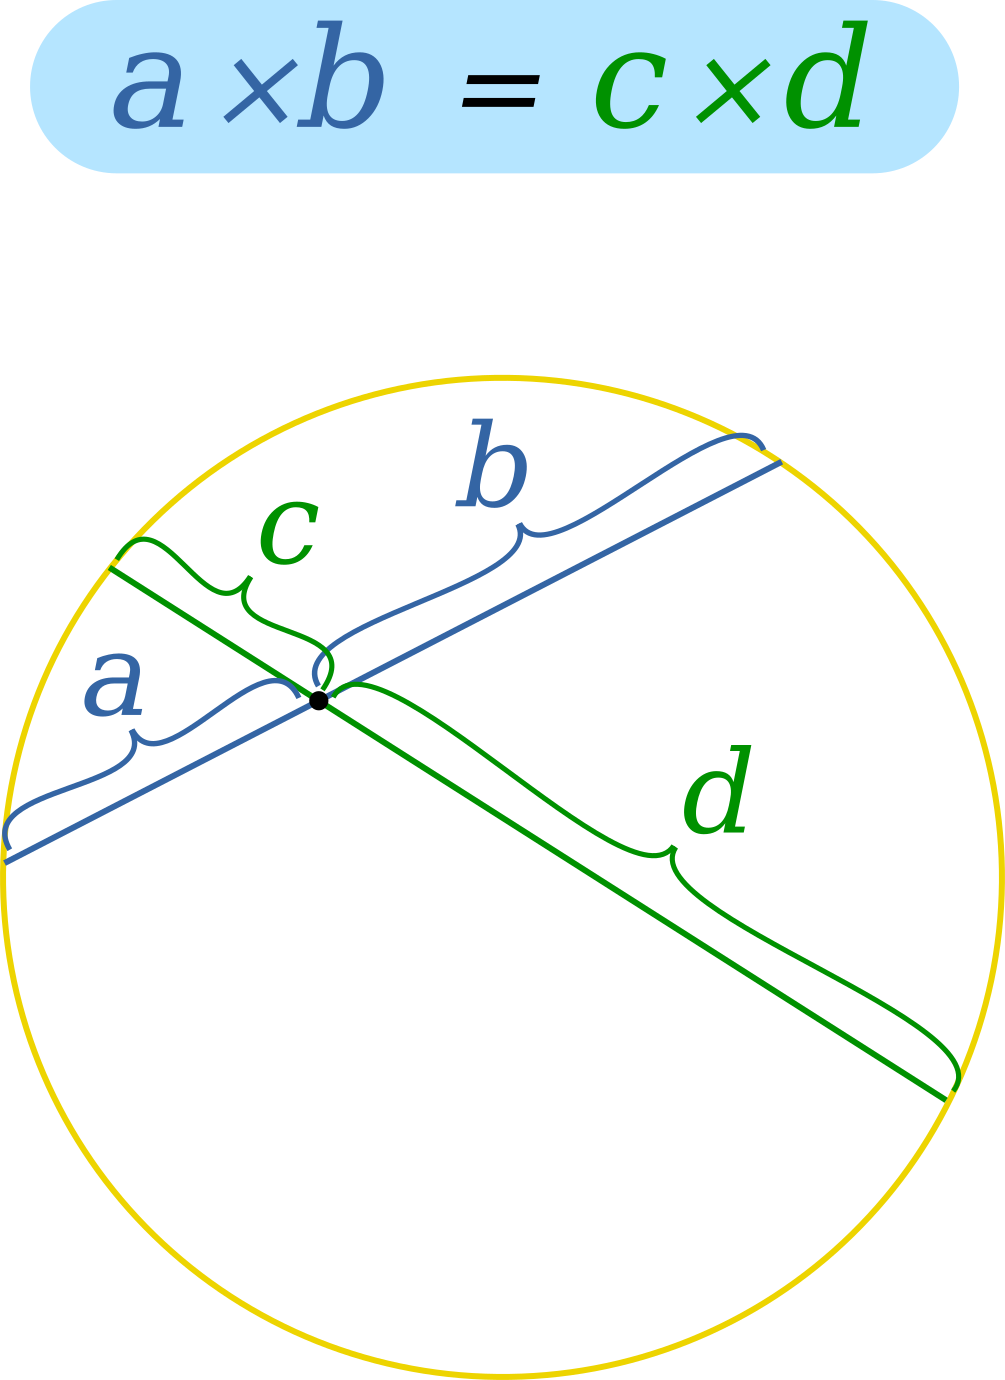
\includegraphics[width=0.5\columnwidth]{teoremacuerdas}
\end{center}
\textbf{Teorema de las Secantes}\\
\begin{center}
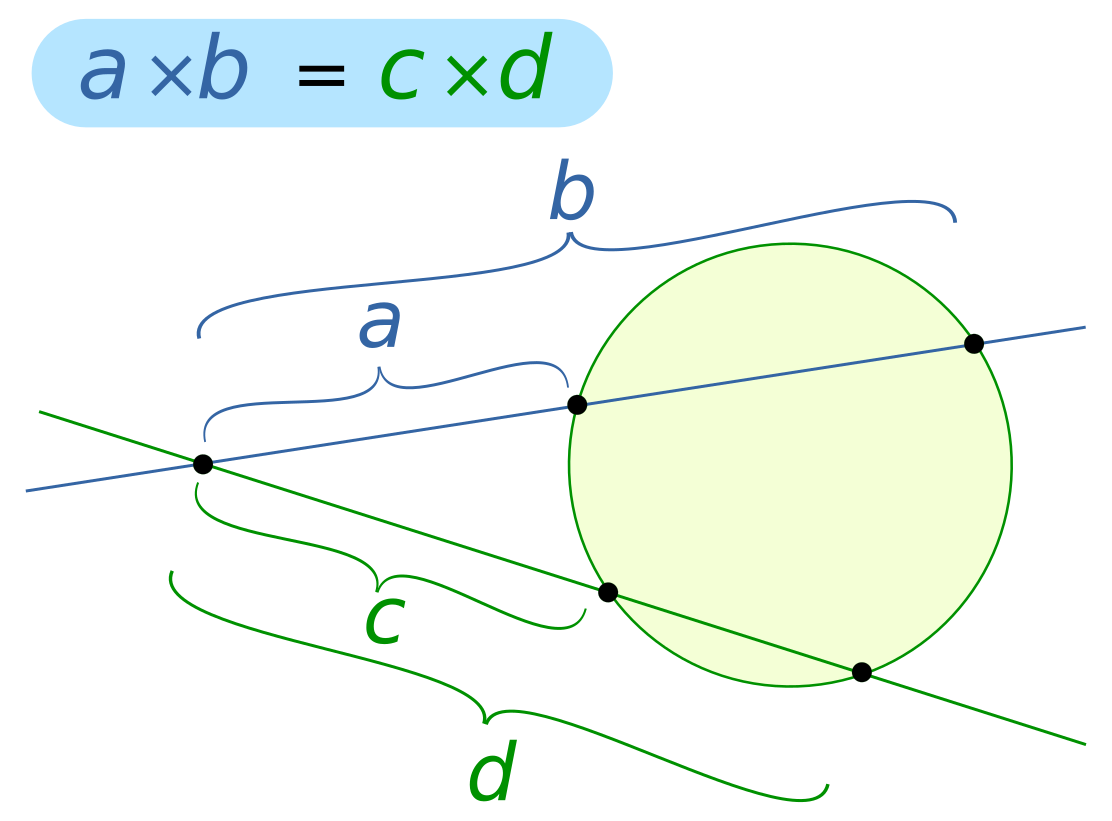
\includegraphics[width=\columnwidth]{teoremasecantes}
\end{center}
\textbf{Teorema de Secante-Tangente}\\
\begin{center}
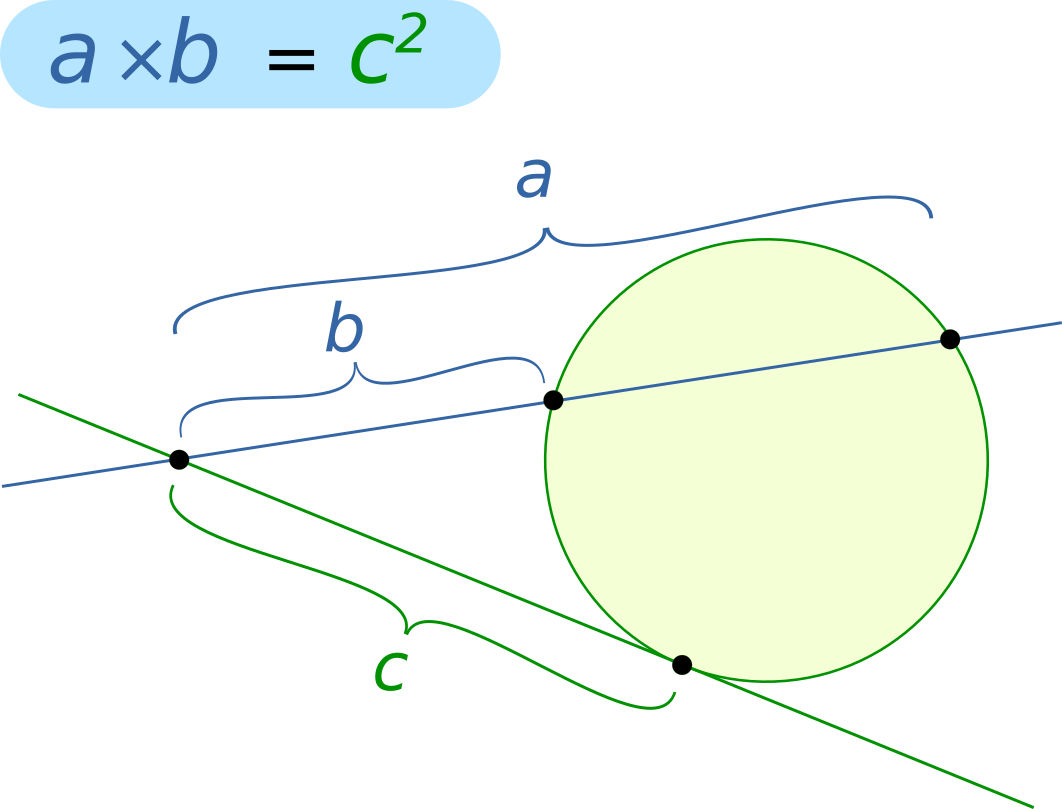
\includegraphics[width=\columnwidth]{teoremasecantetangente}
\end{center}
\vfill\null\columnbreak

\subsection{Rectas y Planos}
Un conjunto de puntos son llamados \textbf{colineales} si pertenecen a una misma recta, lo que puede ser verificado por la igualdad constituida entre las pendientes entre cada par. En álgebra lineal, también se puede verificar comprobando si el área del polígono formado entre los puntos es cero. Trivialmente, todo par de puntos en un plano son colineales, ya que forman una línea.\\

Dos rectas en un mismo plano son llamadas \textbf{coincidentes} si están constituidas por el mismo conjunto de puntos, \textbf{paralelas} si no tienen ningún punto en común (igual pendiente), \textbf{secantes} si solo se intersectam en un punto y \textbf{perpendiculares} si forman entre ellas ángulos rectos ($m_1 \cdot m_2 = -1$).\\

\subsubsection{Teorema de Thales}
Si dos o más \textbf{rectas paralelas} se intersectan por dos transversales, entonces las medidas de los segmentos determinados sobre las secantes son \textbf{proporcionales}.
\begin{center}
\colorbox{white}{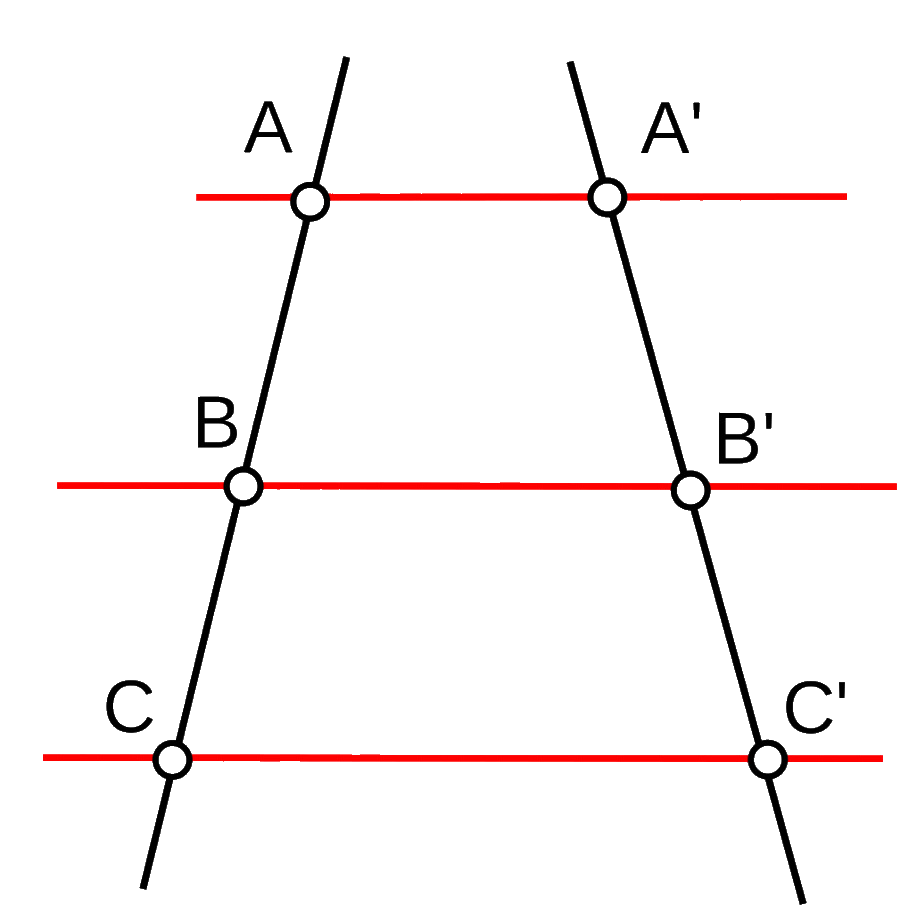
\includegraphics[width=0.5\columnwidth]{teoremathales}}
\end{center}
\subsubsection{Teorema Particular de Thales}
Establece que un segmento de recta paralelo a un lado de un triángulo y que corta a los otros dos, determina en estos últimos segmentos proporcionales. Es importamente mencionar de que el teorema es \textbf{recíproco}.
\begin{center}
    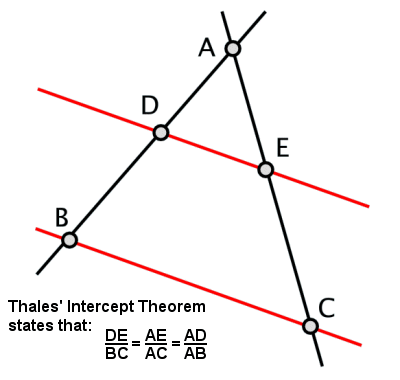
\includegraphics[width=0.8\columnwidth]{teoremathalesparticular}
\end{center}
\subsubsection{Ecuación Vectorial y Paramétrica}
Una recta puede ser expresada en la forma de una \textbf{ecuación vectorial} donde se encuentra definida por un punto de ella, y su dirección. Cualquier vector con la misma dirección (ángulo o pendiente) con respecto a la recta, es llamado \textbf{vector director} ($\vec{d}$), y asimismo un vector de un punto P perteneciente a la recta, es llamado \textbf{vector de posición} ($\vec{P_0}$).\\

De esta forma, la ecuación vectorial de la recta está dada por: \\
$\vec{p} = \vec{p_0} + \lambda\vec{d}$, donde $\lambda \in \mathbb{R}$ y $\vec{p}$ es un vector representando cualquier punto en la recta.

% Intuitivamente, esto significa de que a medida de que $\lambda$ cambia, este modifica la magnitud (por ponderación) de el vector dirección que después es ubicado en el plano por el vector posición.

% Una \textbf{ecuación paramétrica} define un grupo de cantidad como funciones de una o mas variables independientes, llamadas \textbf{parámetros}. Son comúnmente usadas para expresar las coordenadas de puntos que forman objetos geométricos como una curva o una superficie, en cuyo caso se llaman \textit{representaciones parámetricas}.\\

Al resolver la forma general tal que quede expresada en un solo vector, se pueden generar un conjunto de \textbf{ecuaciones paramétricas} (con parámetro $\lambda$) que determinan la recta a través de cada una de sus componentes (como se expresan en el vector resultante).\\

En el plano, la ecuación vectorial puede ser expresada como:

\begin{equation*}
(x, y) = (x_0, y_0) + \lambda(d_x,d_y) \text{ con } \lambda \in \mathbb{R}
\end{equation*}

Y paramétricamente:
\begin{equation*}
    \begin{rcases}
      x = x_0 + \lambda d_x \\
      y = y_0 + \lambda d_y
    \end{rcases}
    \lambda \in \mathbb{R}
    \end{equation*}
Teniendo una ecuación paramétrica, podemos despejar el parámetro ($\lambda$) en cada uno, y despues igualar las expresiones equivalentes del parámetro para obtener una \textbf{ecuación continua} de la forma:
\begin{equation*}
\begin{split}
    \lambda &= \frac{x - x_0}{d_x}\\
    \lambda &= \frac{y - y_0}{d_y}\\
    \frac{x-x_0}{d_x} &= \frac{y-y_0}{d_y}
\end{split}
\end{equation*}
\vfill\null\columnbreak
\subsection{Figuras Planas}
\subsubsection{Congruencia y Semejanza}
Se dice que dos ángulos son congruentes si tienen la misma medida.

De la misma forma, dos segmentos de recta son congruentes si miden lo mismo. \\

Por extensión, dos figuras planas son llamadas \textbf{congruentes} si tienen \textbf{exactamente} la misma forma y tamaño, es decir, si y solo si, todos sus ángulos interiores y lados son congruentes entre sí.
En este contexto, entre dos figuras, los vértices, lados y ángulos que coinciden (homologament)e son llamados \textbf{correspondientes}. La congruencia entre objetos se denota "$\cong$".

Por el otro lado, dos figuras son \textbf{semejantes} ($\sim$) si tienen la misma forma, pero no necesariamente el mismo tamaño (la congruencia es una clase de semejanza), es decir, si todos sus ángulos interiores correspondientes son iguales y la razón entre las medidas de sus lados es constante.\\
\subsubsection{Triángulos}
\textbf{Criterios de Congruencia}\\
\textit{Lado, Lado, Lado (LLL)}: Todos los lados respectivos son congruentes entre ellos.\\
\textit{Lado, Ángulo, Lado (LAL)}: Dos lados respectivos son congruentes, al igual que el ángulo comprendido entre ellos.\\
\textit{Ángulo, Lado, Ángulo (ALA)}: Dos ángulos respectivos son congruentes, al igual que el lado entre ellos.\\

\textbf{Criterios de Semejanza}\\
\textit{Ángulo, Ángulo (AA o AA)}: Todos los ángulos son iguales entre ellos (con dos basta por las propiedades de un triángulo).\\
\textit{Lado, Ángulo, Lado (LAL)}: Dos lados tienen medidas \textbf{proporcionales} y los ángulos comprendidos entre ellos son congruentes.\\
\textit{Lado, Lado, Lado (LLL)}: Todos los lados correspondientes son \textbf{proporcionales}, es decir hay una constante para la relación entre cada par de lados.\\
\vfill\null\columnbreak
\textbf{Teorema de Euclides}\\
En un triángulo \textbf{rectángulo}, la altura de la hipotenusa divide al triángulo en dos triángulos semejantes entre ellos, al igual que semejantes al triángulo original. De esto se deriva que el cuadrado de tal altura es igual al producto entre las protecciones de los catetos sobre la hipotenusa:
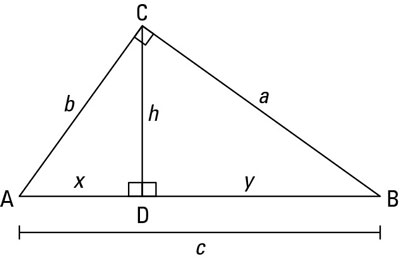
\includegraphics[width=\columnwidth]{euclides}
\begin{equation*}
{h_c}^2 = x \cdot y
\end{equation*}
También de esto se deriva que el cuadrado de un cateto es igual al producto de la hipotenusa y su proyección del cateto.

\begin{equation*}
    a^2 = c \cdot x; b^2 = c \cdot y
\end{equation*}
\textbf{Teorema de Pitagoras}\\
En un triángulo \textbf{rectángulo}, el área del cuadrado construido sobre la hipotenusa es igual a la suma de las áreas de los cuadrados sobre los catetos.
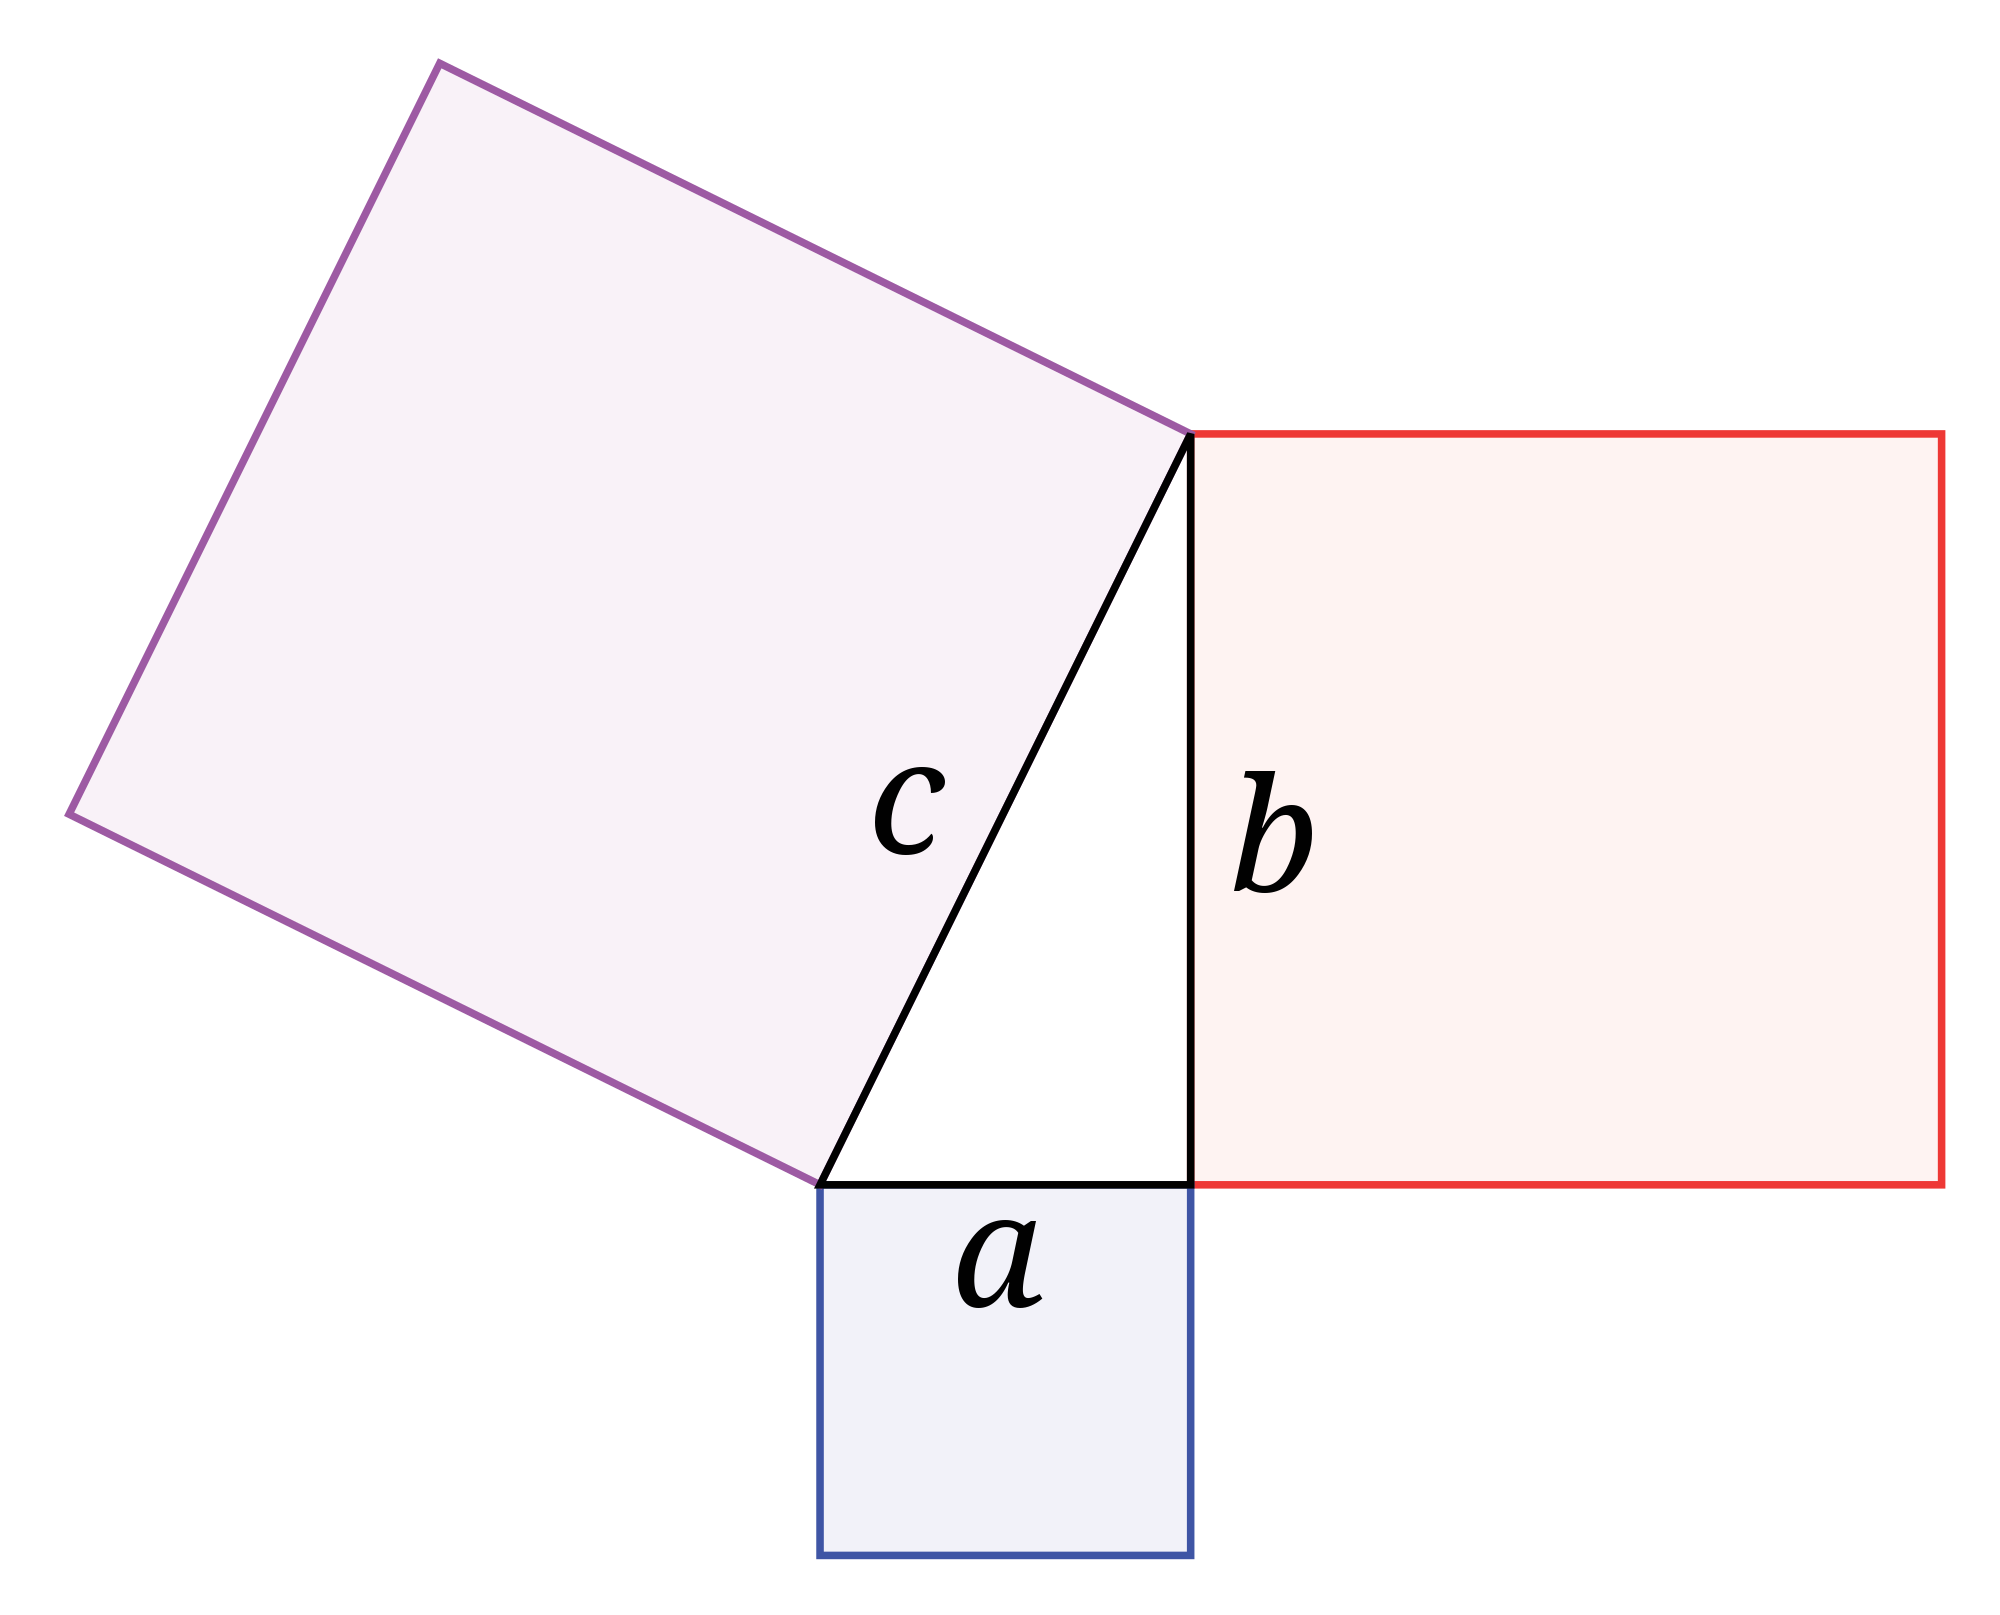
\includegraphics[width=\columnwidth]{pitagoras}

De esto deriva la \textbf{ecuación pitagórica}:
\begin{equation*}
    a^2 + b^2 = c^2
\end{equation*}
Es importante notar que esta es un teorema \textbf{recíproco}, es decir, cuando esta ecuación se cumple en un triángulo dado se puede afirmar que es rectángulo.\\
\vfill\null\columnbreak
\subsection{Cuerpos Geométricos}
Se denominan \textbf{cuerpos o sólidos de revolución} a aquellos objetos geométricos que pueden obtenerse mediante la rotación de una figura plana alrededor de una recta denominada eje. (en un espacio tridimensional, \textit{e.j} un cilindro recto por rotación de un rectángulo, una esfera por un semicirculo, un cono por un triangulo rectángulo y un cono truncado por un trapecio rectángulo.)\\

Por el otro lado, un \textbf{cuerpo de traslación} es uno obtenido mediante la traslación de una figura plana. (\textit{e.j} el prisma recto, generado por un polígono trasladado perpendicular a su plano; el cilindro recto generado por la traslación de un círculo).
\subsubsection{Prisma}
Un prisma es un cuerpo geométrico con dos caras paralelas y congruentes llamadas bases, con la restantes caras laterales siendo paralelogramos. Se nombran según los polígonos de sus bases. \\
\begin{equation*}
    \begin{split} 
    A_{\text{lateral}} &= h \cdot P_b\\
    A_{\text{total}} &= 2\cdot A_b + A_l\\
    V &= A_b\cdot h
    \end{split}
\end{equation*}

\subsubsection{Pirámide}
Las pirámides son cuerpos que tienen como base un polígono cualquiera y sus caras laterales concurren en un punto llamado cúspide. Se nombran según el polígono de su base.\\
\begin{equation*}
    \begin{aligned} 
    V = \frac{1}{3}A_b\cdot h
    \end{aligned}
\end{equation*}
\subsubsection{Cilindro}
El cilindro recto es el cuerpo generado al girar un rectángulo en torno a la recta que contiene a uno de sus lados, o bien al traslador un círculo de forma perpendicular a un plano que contiene la base. Este cuerpo queda limitado por una superficie curva llamado manto (label) y dos supericies planas circulares, llamadas bases.

\begin{equation*}
    \begin{split} 
    A_{\text{lateral}} &= 2\pi rh\\
    A_{\text{basal}} &= \pi r^2\\
    A_{\text{total}} &= 2\pi rh + 2\pi ^2 \equiv 2\pi r(h+r)\\
    V &= \pi r^2h
    \end{split}
\end{equation*}
\subsubsection{Cono}
Un cono recto es el cuerpo generado al girar un triángulo rectángulo en torno a la recta que contiene uno de sus catetos. La hipotenusa de tal triángulo se llama generatriz. ($g$)

\begin{equation*}
    \begin{split} 
        &g = \sqrt{r^2 + h^2}\\
        A_{\text{total}} &= A_b + A_l = \pi r^2 + \pi rg \\
        &= \pi r(r + \sqrt{r^2 + h^2}
    \end{split}
\end{equation*}
\begin{equation*}
    \begin{aligned} 
        V = \frac{1}{3}\pi r^2h
    \end{aligned}
\end{equation*}
\subsubsection{Esfera}
La esfera es el cuerpo generado al girar un semicírculo en torno a la recta que contiene al díametro. También puede ser descrito como un conjunto de todos los puntos en el espacio cuya distancia a un punto fijo, llamado centro, es menor o igual a su radio.

\begin{equation*}
    \begin{split} 
        A &= 4\pi r^2\\
        V &= \frac{4}{3} \pi r^3
    \end{split}
\end{equation*}
\vfill\null\columnbreak